\chapter{Verfahren} \chaplabel{verfahren}

In den folgenden Abschnitten wird das Verfahren erläutert, welches das Lernen von Bewegungsdaten eines Datenhandschuhs ermöglicht. Zunächst wird der Systemaufbau erklärt und der verwendete Datenhandschuh vorgestellt. Dabei wird jedoch auf eine detaillierte Beschreibung der Entwicklung des Handschuhs verzichtet. Die genauen Details sind in der Arbeit von Paul \citet{paul} beschrieben.

Desweiteren werden die verwendeten Python-Bibliotheken vorgestellt und die Datenvorverarbeitung sowie das Einteilen der Daten in geeignete Abschnitte erläutert.

Schließlich werden die benutzten Methoden des maschinellen Lernens vorgestellt.

\section{Systemaufbau}

Der Datenhandschuh misst mit den an den Fingern positionierten Sensoren die Beschleunigung (Accelerometer), die Rotationsgeschwindigkeit (Gyroskop) und das Erdmagnetfeld (Magnometer). Diese Daten werden zu sogenannten \fremdwort{Quaternionen}\footnote{Quaternionen sind ein mathematisches Konstrukt, nützlich um die Orientierung von Objekten im Raum oder Drehungen zu beschreiben.} fusioniert, welche wir für das Lernen verwenden.

In \figref{overview} sind die Komponenten unseres Systems abgebildet.
Die Daten der sechs IMUs werden mithilfe von drei \iic-Bussen zum Mikroprozessor übertragen. Über WLAN oder USB-Kabel werden die Daten an den Computer geleitet. Es gibt zwei mögliche Modi, den Lernmodus (gestrichelte Linien) und den Anwendungsmodus (durchgezogene Linien).

Im Lernmodus werden die Sensordaten vom \fremdwort{Serial Parser} und die Tastendrücke vom \fremdwort{Keyboard Listener} in ein \fremdwort{ROS-Bag} gespeichert. Das \fremdwort{Robot Operating System} (ROS)~\cite{web:ros} ist eine Sammlung von Bibliotheken und Werkzeugen für die Entwicklung von Robotersystemen.

Für die Vorverarbeitung (\fremdwort{Preprocessing}) werden die Daten dann aus dem ROS-Bag gelesen. Die Vorverarbeitung dient unter anderem der Reduzierung der Datendimensionalität. Zudem werden die benötigten Daten zu regelmäßigen Zeitpunkten ermittelt, die durch das zeitversetzte Senden der IMUs eventuell nicht direkt vorliegen. Nach dem Vorverarbeiten werden die Daten dann in geeignete Samples geteilt. Jedes Sample besteht hierbei aus einer festen Anzahl an Zeitschritten und enthält jeweils einen Tastendruck. Außerdem werden Samples für die Klasse $\emptyset$, also ,,keine Taste gedrückt'', angelegt. Das \fremdwort{Sampling} dient dazu, einheitliche, zeitdiskrete Daten an das neuronale Netz zu geben.

Beim \fremdwort{Learning} werden die Samples von dem Netz gelernt, die gelernten Netzparameter bilden das Modell und werden gespeichert, um sie später anwenden zu können.

Im Anwendungsmodus werden die Lernschritte ausgelassen. Die Daten werden zwar immer noch in Samples geteilt, diese werden jedoch nicht mehr gezielt ausgesucht. Stattdessen wird jeweils eine feste Anzahl der zuletzt eingetroffenen Zeitschritte als ein Sample zusammengefasst und ausgewertet. Dadurch entsteht ein gleitendes Zeitfenster, einzelne Datenpunkte sind in mehreren Samples enthalten. Für das Anwenden werden die im Vorfeld gelernten Netzparameter geladen. Die vom Netz getätigten Ausgaben werden an das Betriebssystem weitergegeben und als Tastatureingaben interpretiert.

\begin{figure}
    \centering
    \begin{tikzpicture}[
    onslide/.code args={<#1>#2}{%
        \ifdefined\only
        \only<#1>{\pgfkeysalso{#2}}%
        \else
        #2
        \fi
    },
    every node/.style={
        font=\small,
        inner sep=0pt,
        thick,
    },
    node distance=2cm,
    database/.style={
        cylinder,
        shape border rotate=90,
        aspect=0.2,
        draw,
        minimum width=2.5cm,
        text width=2.5cm,
        align=center,
        minimum height=1.5cm,
    },
    node/.style={
        rectangle,
        draw,
        text width=2.5cm,
        align=center,
        minimum height=1cm,
        rounded corners=2pt,
    },
    arrow/.style={
        thick,
        ->,
        >=stealth,
    },
    learning/.style={
        dashed,
    },
    applying/.style={
        very thick,
    },
    radiation/.style={
        decorate,
        decoration={expanding waves,angle=10,segment length=4pt}
    },
    wire/.style={
        % draw=gray,
    },
    sensor/.style={
        node,
        minimum width=5mm,
        minimum height=5mm,
        text width=0,
        draw,
        rectangle,
        rounded corners=0,
    },
    highlight/.style={
        draw=primary,
        color=primary,
        fill=primary!10!white,
    },
    drawhighlight/.style={
        thick,
        draw=primary,
    },
    texthighlight/.style={
        color=primary,
    },
]

    \coordinate (legend) at (6.5, 0.2);
    \draw[thick,wire]           ($ (legend) + (0,    0) $) -- node[at end, right, xshift=0.2cm] {Wire}  ++(0.5, 0);
    \draw[thick,arrow,learning] ($ (legend) + (0, -0.6) $) -- node[at end, right, xshift=0.2cm] {Learn} ++(0.5, 0);
    \draw[thick,arrow,applying] ($ (legend) + (0, -1.2) $) -- node[at end, right, xshift=0.2cm] {Apply} ++(0.5, 0);
    \draw ($ (legend) + (-0.2, 0.3) $) rectangle ++(2, -1.8);

    \node[node]
        (serialparser)
        at (0, 0)
        {Serial Parser};

    \node[node,left=2cm of serialparser]
        (sender)
        {Micro-\\processor};

    \node[sensor,below left=7mm and 0.5cm of sender.south]  (sensor1) {};
    \node[sensor,below=2mm of sensor1] (sensor2) {};
    \node[sensor,below=2mm of sensor2] (sensor3) {};
    \node[sensor,below right=7mm and 0.5cm of sender.south] (sensor4) {};
    \node[sensor,below=2mm of sensor4] (sensor5) {};
    \node[sensor,below=2mm of sensor5] (sensor6) {};

    \node[below=3cm of sender] {Sensors};
    \draw[wire,onslide={<2> drawhighlight}] (sensor1) -| ($ (sender.south) + (-0.2, 0) $);
    \draw[wire,onslide={<2> drawhighlight}] (sensor2) -| ($ (sender.south) + (-0.12, 0) $);
    \draw[wire,onslide={<2> drawhighlight}] (sensor3) -| ($ (sender.south) + (-0.04, 0) $);
    \draw[wire,onslide={<2> drawhighlight}] (sensor4) -| ($ (sender.south) + (0.2, 0) $);
    \draw[wire,onslide={<2> drawhighlight}] (sensor5) -| ($ (sender.south) + (0.12, 0) $);
    \draw[wire,onslide={<2> drawhighlight}] (sensor6) -| ($ (sender.south) + (0.04, 0) $);

    \draw[radiation,onslide={<3> drawhighlight}]
        ([xshift=2mm,yshift=-0.3cm]sender.east) -- node[midway,yshift=-0.6cm,onslide={<3> texthighlight}] {or WiFi} ([xshift=-2mm,yshift=-0.3cm]serialparser.west);

    \draw[very thick,wire,onslide={<3> drawhighlight}]
        ([yshift=0.2cm]sender.east) -- node[midway,yshift=0.3cm,onslide={<3> texthighlight}] {USB} ([yshift=0.2cm]serialparser.west);

    \node[node,right=1cm of serialparser]
        (keyboard)
        {Keyboard\\Listener};

    \node[database]
        (bag)
        at ($ (serialparser) + (1.75, -2) $)
        {ROS Bag};

    \node[node,text width=6cm,onslide={<5> highlight}]
        (preprocessing)
        at ($ (serialparser) + (1.75, -4) $)
        {Preprocessing};

    \node[node, below=1cm of preprocessing.south west,anchor=north west,onslide={<5> highlight}]
        (apply)
        {Apply\\Network};

    \node[database, below=1.5cm of preprocessing.south east,anchor=east,onslide={<5> highlight}]
        (model)
        {Saved Model};

    \node[node, right=1cm of preprocessing,onslide={<5> highlight}]
        (sampling)
        {Sampling};

    \node[node, below=1cm of sampling,onslide={<5> highlight}]
        (learning)
        {Learning};

    \node[node, text width=9.5cm]
        (os)
        at ($ (apply) + (3.5, -2) $)
        {Operating System};

    \draw [arrow,applying] ($ (serialparser) + (-0.5,-0.5) $) -- +(0, -3);
    \draw [arrow,learning] ($ (serialparser) + (0,-0.5) $) -- +(0, -1) -- (bag);
    \draw [arrow,learning] ($ (keyboard) + (0,-0.5) $) -- +(0, -1) -- (bag);
    \draw [arrow,learning] (bag) -- (preprocessing);
    \draw [arrow,applying] ($ (preprocessing) + (-2.25,-0.5) $) -- +(0, -1);
    \draw [arrow,applying] (model) -- (apply);
    \draw [arrow,learning] (preprocessing) -- (sampling);
    \draw [arrow,learning] (sampling) -- (learning);
    \draw [arrow,learning] (learning) -- (model);
    \draw [arrow,applying] ($ (apply) + (-0.5,-0.5) $) -- +(0, -1);

    \draw[dotted,line width=2pt] ($ (serialparser) !.5! (sender) + (0, -1.5) $) -- node[at end] (bottom) {} +(0, -8);
    \draw[dotted,line width=2pt] ($ (serialparser) !.5! (sender) + (0, 1) $) -- +(0, 0.5);

    \node[anchor=north west,right=10mm of bottom,yshift=0.5em] {\large{}\textbf{HOST PC}};
    \node[anchor=north east,left=10mm of bottom,yshift=0.5em] {\large{}\textbf{GLOVE}};

    \ifdefined\setbeamertemplate
        \only<1-4>{
            \node[node, anchor=north west, minimum width=9.6cm, minimum height=3.2cm, fill=white] at (preprocessing.north west) {Machine learning};
        }
    \fi
\end{tikzpicture}

    \caption[Aufbau des Systems]{Aufbau des Systems. Die Sensoren zeichnen Daten auf, welche vom Mikroprozessor entweder über USB oder über WLAN an den \fremdwort{Serial Parser} übermittelt werden. Im Lernmodus werden die Daten mitsamt der dazugehörigen Tastendrücke aus dem \fremdwort{Keyboard Listener} in ein \fremdwort{ROS-Bag} gespeichert. Nach der Vorverarbeitung und der Einteilung in geeignete Samples wird ein neuronales Netz anhand der Daten trainiert und das gelernte Modell gespeichert. Im Anwendungsmodus werden die Lernschritte übersprungen und das bereits gelernte Netz geladen, um nach dem Vorverarbeiten der Daten diese zu klassifizieren.}
    \figlabel{overview}
\end{figure}

\subsection{Der Datenhandschuh}

\begin{figure}[htb]
    \begin{subfigure}[t]{0.59\textwidth}
        \centering
        \fbox{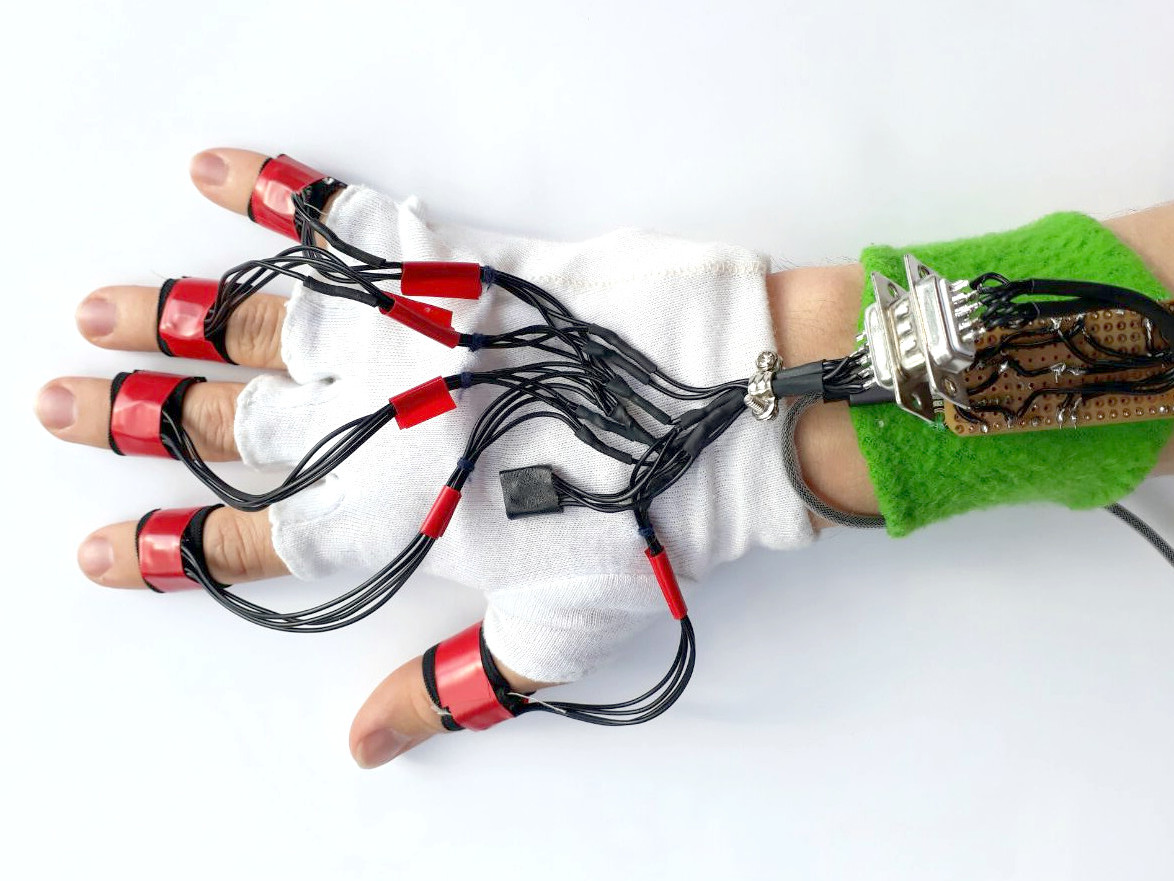
\includegraphics[height=6cm]{../common/images/glove-sideways}}
        \caption{Fertiggestellter Handschuh mit 6 IMUs auf den Fingern und dem Handrücken. Der Mikroprozessor wird durch eine Steckverbindung mit den IMUs verbunden.}
        \figlabel{photos:finished-glove}
    \end{subfigure}
    \hfill
    \begin{subfigure}[t]{0.4\textwidth}
        \centering
        \fbox{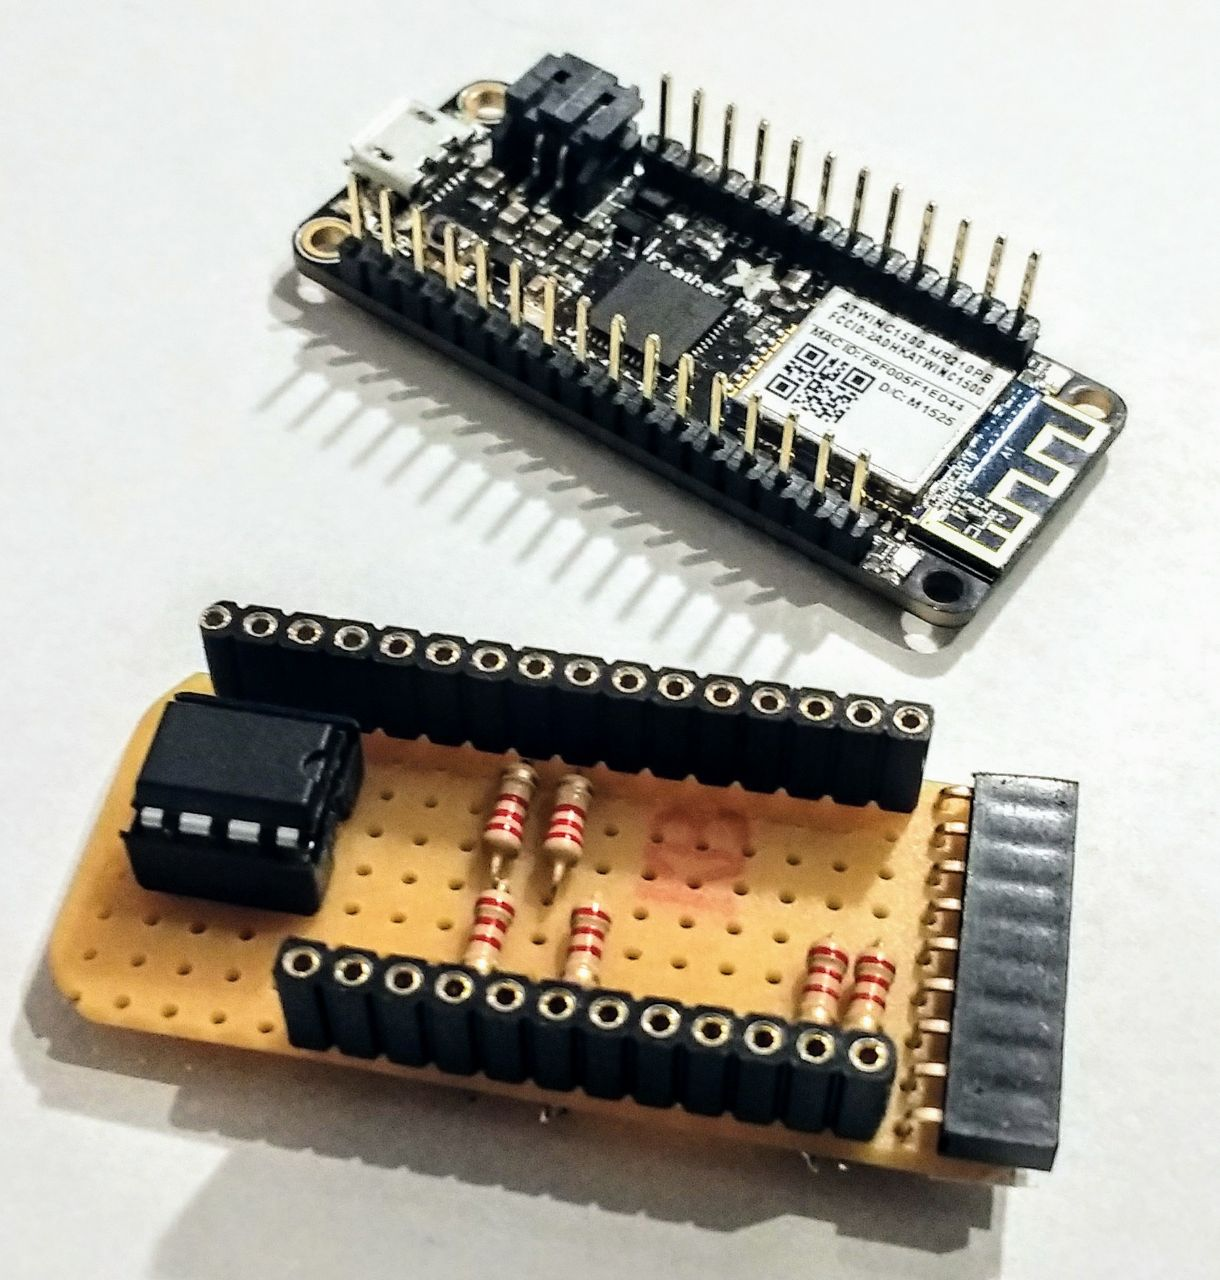
\includegraphics[height=6cm]{../common/images/shield}}
        \caption{Featherboard mit Entwicklungsplatine; die Platine wird auf den Mikroprozessor aufgesteckt. Diese enthält dem Mikroprozessor fehlende Widerstände und ein EEPROM. Durch die Platine wird zudem die Verkabelung vereinfacht.}
        \figlabel{photos:shield}
    \end{subfigure}

    \caption[Prototyp des Datenhandschuhs mit den einzelnen Komponenten]{Hier ist der Prototyp des Datenhandschuhs mit den einzelen Komponenten abgebildet.}
    \figlabel{photos}
\end{figure}

Der fertige Datenhandschuh ist in \figref{photos} zu sehen. Er besteht aus

\begin{itemize}
    \item sechs Inertial Measurement Units (IMUs) des Typs \productname{BNO055}, befestigt an den Fingern und dem Hand\-rücken,
    \item einem fingerlosen dünnen Baumwollhandschuh zur Befestigung der Hand-IMU,
    \item 5 Ringen aus elastischem Textilband zur Befestigung der IMUs am zweiten Segment der Finger,
    \item dem Mikroprozessor \productname{Adafruit Feather M0 WiFi} (,,Featherboard''),
    \item einer Entwicklungsplatine, welche auf den Mikroprozessor gesteckt wird und sowohl die Verkabelung vereinfacht, als auch Platz für ein EEPROM und die benötigten Pull-Up-Widerstände bietet,
    \item einem breiten Band ums Handgelenk, auf welchem der Mikroprozessor mit der Entwicklungsplatine befestigt ist, sowie
    \item einer Steckverbindung und diversen Kabeln zur Verbindung der Komponenten.
\end{itemize}

Die IMUs enthalten jeweils ein Accelerometer, ein Gyroskop und einen 3D-Kompass (Magnetometer). Außerdem ist ein Mikroprozessor mit einem vorinstallierten Fusionsalgorithmus enthalten, mit dessen Hilfe die IMU die einzelnen Sensordaten zu einer Quaternion fusioniert. Diese Quaternion gibt die absolute Orientierung des Sensors im Raum an.

\subsection{Datenübertragung}

Die IMUs erfassen die Bewegungen der Finger und der Hand. Diese Daten werden über einen \iic-Bus vom Featherboard ausgelesen. Da die IMUs über jeweils 2 verschiedene Adressen ansprechbar sind, reichen die insgesamt 3 freien \iic-Busse des Featherboards aus. Vom Featherboard werden die IMU-Daten in einzelnen Paketen an den Host-PC übermittelt. Jedes Paket enthält die Accelerometer- und Gyroskopdaten sowie die fusionierte Quaternion. Dies ergibt pro Paket 10 Werte mit insgesamt 20 Bytes. Die Pakete können seriell per USB oder über WLAN und UDP übermittelt werden.

Mithilfe eines in Python geschriebenen Parsers werden die Pakete dann in ROS-Nach\-rich\-ten verwandelt. Dies ermöglicht ein leichtes Aufzeichnen und späteres Verwenden der Daten, um mit diesen zeitlich unabhängig lernen zu können. Ein Live-Betrieb zur Anwendung des gelernten Modells ist ebenfalls möglich.

\section{Bibliotheken für maschinelles Lernen}

Für das Arbeiten mit neuronalen Netzen gibt es einige Frameworks und Bibliotheken, um die Anforderungen an die Komplexität der Netze leichter erfüllen zu können.
Wir haben uns für die Kombination aus Theano \citep{theano} und Lasagne~\cite{web:lasagne} entschieden.

Theano ist eine open-source Python-Bibliothek, die auf komplexe und große wissenschaftliche Berechnungen ausgelegt ist und auf NumPy \citep{numpy} basiert. Wir nutzen NumPy zudem für einfache Datenverarbeitungsschritte, wie beispielsweise beim Vorverarbeiten. Theano optimiert Berechnungen mit multi-dimensionalen Arrays mit einem Fokus auf Effizienz und Schnelligkeit. Desweiteren ermöglicht Theano ohne großen Aufwand eine Ausführung der Berechnung auf einer oder mehreren CPUs oder sogar auf GPUs. Hierfür muss lediglich eine entsprechende Umgebungsvariable gesetzt werden:

\begin{listing}[h]
    \inputminted{bash}{../common/code/theano-flags.sh}
    \caption[Umgebungsvariable in Theano um Ausführungsziel zu bestimmen]{Theano Umgebungsvariablen zur Steuerung des Ausführungsziels. Durch das Setzen dieser kann entschieden werden, ob auf einer GPU oder einer oder mehreren CPUs gelernt werden soll.}
    \lstlabel{theano-flags}
\end{listing}

Lasagne ist eine auf Theano basierende Bibliothek, die auf neuronale Netze spezialisiert ist. Mit Hilfe von Lasagne ist es leicht möglich, verschiedene Arten von Schichten eines neuronalen Netzes als Theano-Formeln zu konfigurieren. Zudem kann das Gesamtnetz ohne große Komplikationen initialisiert, trainiert und schließlich auch angewendet werden.
Außerdem ist es ist mithilfe von Lasagne, Theano und NumPy auch möglich, die gelernten Netzparameter zu serialisieren, sodass gelernte Netze leicht gespeichert und später für weitere Nutzung geladen werden können. Lasagne formulierte alle Netzwerkoperationen so, dass Stapelverarbeitung mehrerer Samples leicht möglich ist.

Das Verwenden von Lasagne soll hier anhand eines sehr einfachen CNN vorgestellt werden:

\begin{listing}[h]
    \inputminted{python}{../common/code/lasagne.py}
    \caption[CNN in Lasagne]{Modellierung eines einfachen CNN in Lasagne mit einer Eingabeschicht, einigen Convolution/Pooling-Schicht-Paaren und schließlich einer Ausgabeschicht.}
    \lstlabel{lasagne-cnn}
\end{listing}

Zunächst wird eine Eingabeschicht erzeugt. Das \texttt{shape}-Argument beschreibt die Dimensionalität der Eingabedaten. Hierbei bleibt die erste Dimension \texttt{None}, dadurch wird die Stapelgröße anhand der Eingabedaten ermittelt. Ein Stapel besteht in der Regel aus mehreren Samples, um die Berechnung zu beschleunigen.

In der Schleife werden die Convolution- und Max-Pooling-Schichten angelegt. Die Größen \texttt{FILTER\_SIZE} und \texttt{FILTER\_COUNT} geben die Dimension und die Anzahl der genutzten Filter an, die \texttt{POOLING\_SIZE} bestimmt die Größe der Region, aus welcher im Pooling-Schritt der größte Wert übernommen wird.

Um die Reihenfolge der Schichten zu definieren, wird die aktuelle Schicht in einer Variable gespeichert und in der nächsten Schicht als Vorgänger angegeben.

Schließlich wird die vollständig verknüpfte Ausgabeschicht (\fremdwort{dense layer}) ans Ende des Netzes gestellt.

\section{Vorverarbeitung}

Bevor die Daten an das neuronale Netz gegeben werden, werden sie vorverarbeitet. Ziel der Vorverarbeitung ist es, die wichtigen Informationen besser zugänglich zu machen und die zu evaluierende Datenmenge zu reduzieren.

Wir gehen zunächst davon aus, dass die Quaternionen bereits einen guten Überblick über die Bewegungsabläufe der verschiedenen Tastendrücke geben, weshalb wir zu Beginn ausschließlich diese verwenden und auf die rohen Sensorwerte des Accelerometers und des Gyroskops verzichten. Dies spart uns Komplexität im Modell, und wir müssen uns zudem nicht um eine geeignete Kalibrierung während des Tippens kümmern.

\begin{figure}[htb]
    \centering
    \begin{tikzpicture}[
    node distance=5mm,
    node/.style={
        flowchart node,
        minimum width=2cm,
        text width=2cm,
    },
]
    \node[node]  (quat) at (0, 0) {Absolute Quaternionen};
    \node[node, right=of quat] (rel) {Relativ zur Handbasis};
    \node[node, right=of rel] (int) {Zeitschritt/\\Interpolation};
    \node[node, right=of int] (samples) {Sampling};
    \node[node, right=of samples,dashed] (angles) {Euler-Winkel visualisieren};

    \draw[flowchart arrow] (quat) -- (rel);
    \draw[flowchart arrow] (rel) -- (int);
    \draw[flowchart arrow] (int) -- (samples);
    \draw[flowchart arrow,dashed] (samples) -- (angles);
\end{tikzpicture}

    \caption{Schritte des Preprocessings}
    \figlabel{preprocessing}
\end{figure}

Wie in \figref{preprocessing} zu sehen, beginnen wir bei der Vorverarbeitung damit, dass wir ausschließlich die Quaternionen nutzen. Durch das Ignorieren der Beschleunigung und der Rotationsgeschwindigkeit gehen zwar nützliche Informationen verloren, es reduziert jedoch auch drastisch die Datenmenge. Da es sich in diesem Projekt um einen Prototyp handelt ist dies von großem Nutzen, denn Ergebnisse sind so schneller zu erzielen. In der Zukunft wird es sich höchstwahrscheinlich als sinnvoll erweisen, die bisher ungenutzten Daten wieder mit einzubeziehen, vor allem wenn mit dem Handschuh immer größere Bewegungen ermöglicht werden sollen, um weit entfernte Tasten drücken zu können, oder auch um verschiedene Gesten durchführen zu können.

% Beim Visualisieren der IMU-Daten fällt ein weiteres Problem auf: Die IMUs stehen in keinem Bezug zueinander. Dies erschwert das Lernen und verhindert zudem, dass die Benutzung des Datenhandschuhs von der Orientierung der Testperson abhängig ist, da Quaterniondaten ausrichtungssensibel sind.

\begin{figure}
    \centering
    \begin{subfigure}[t]{0.49\textwidth}
        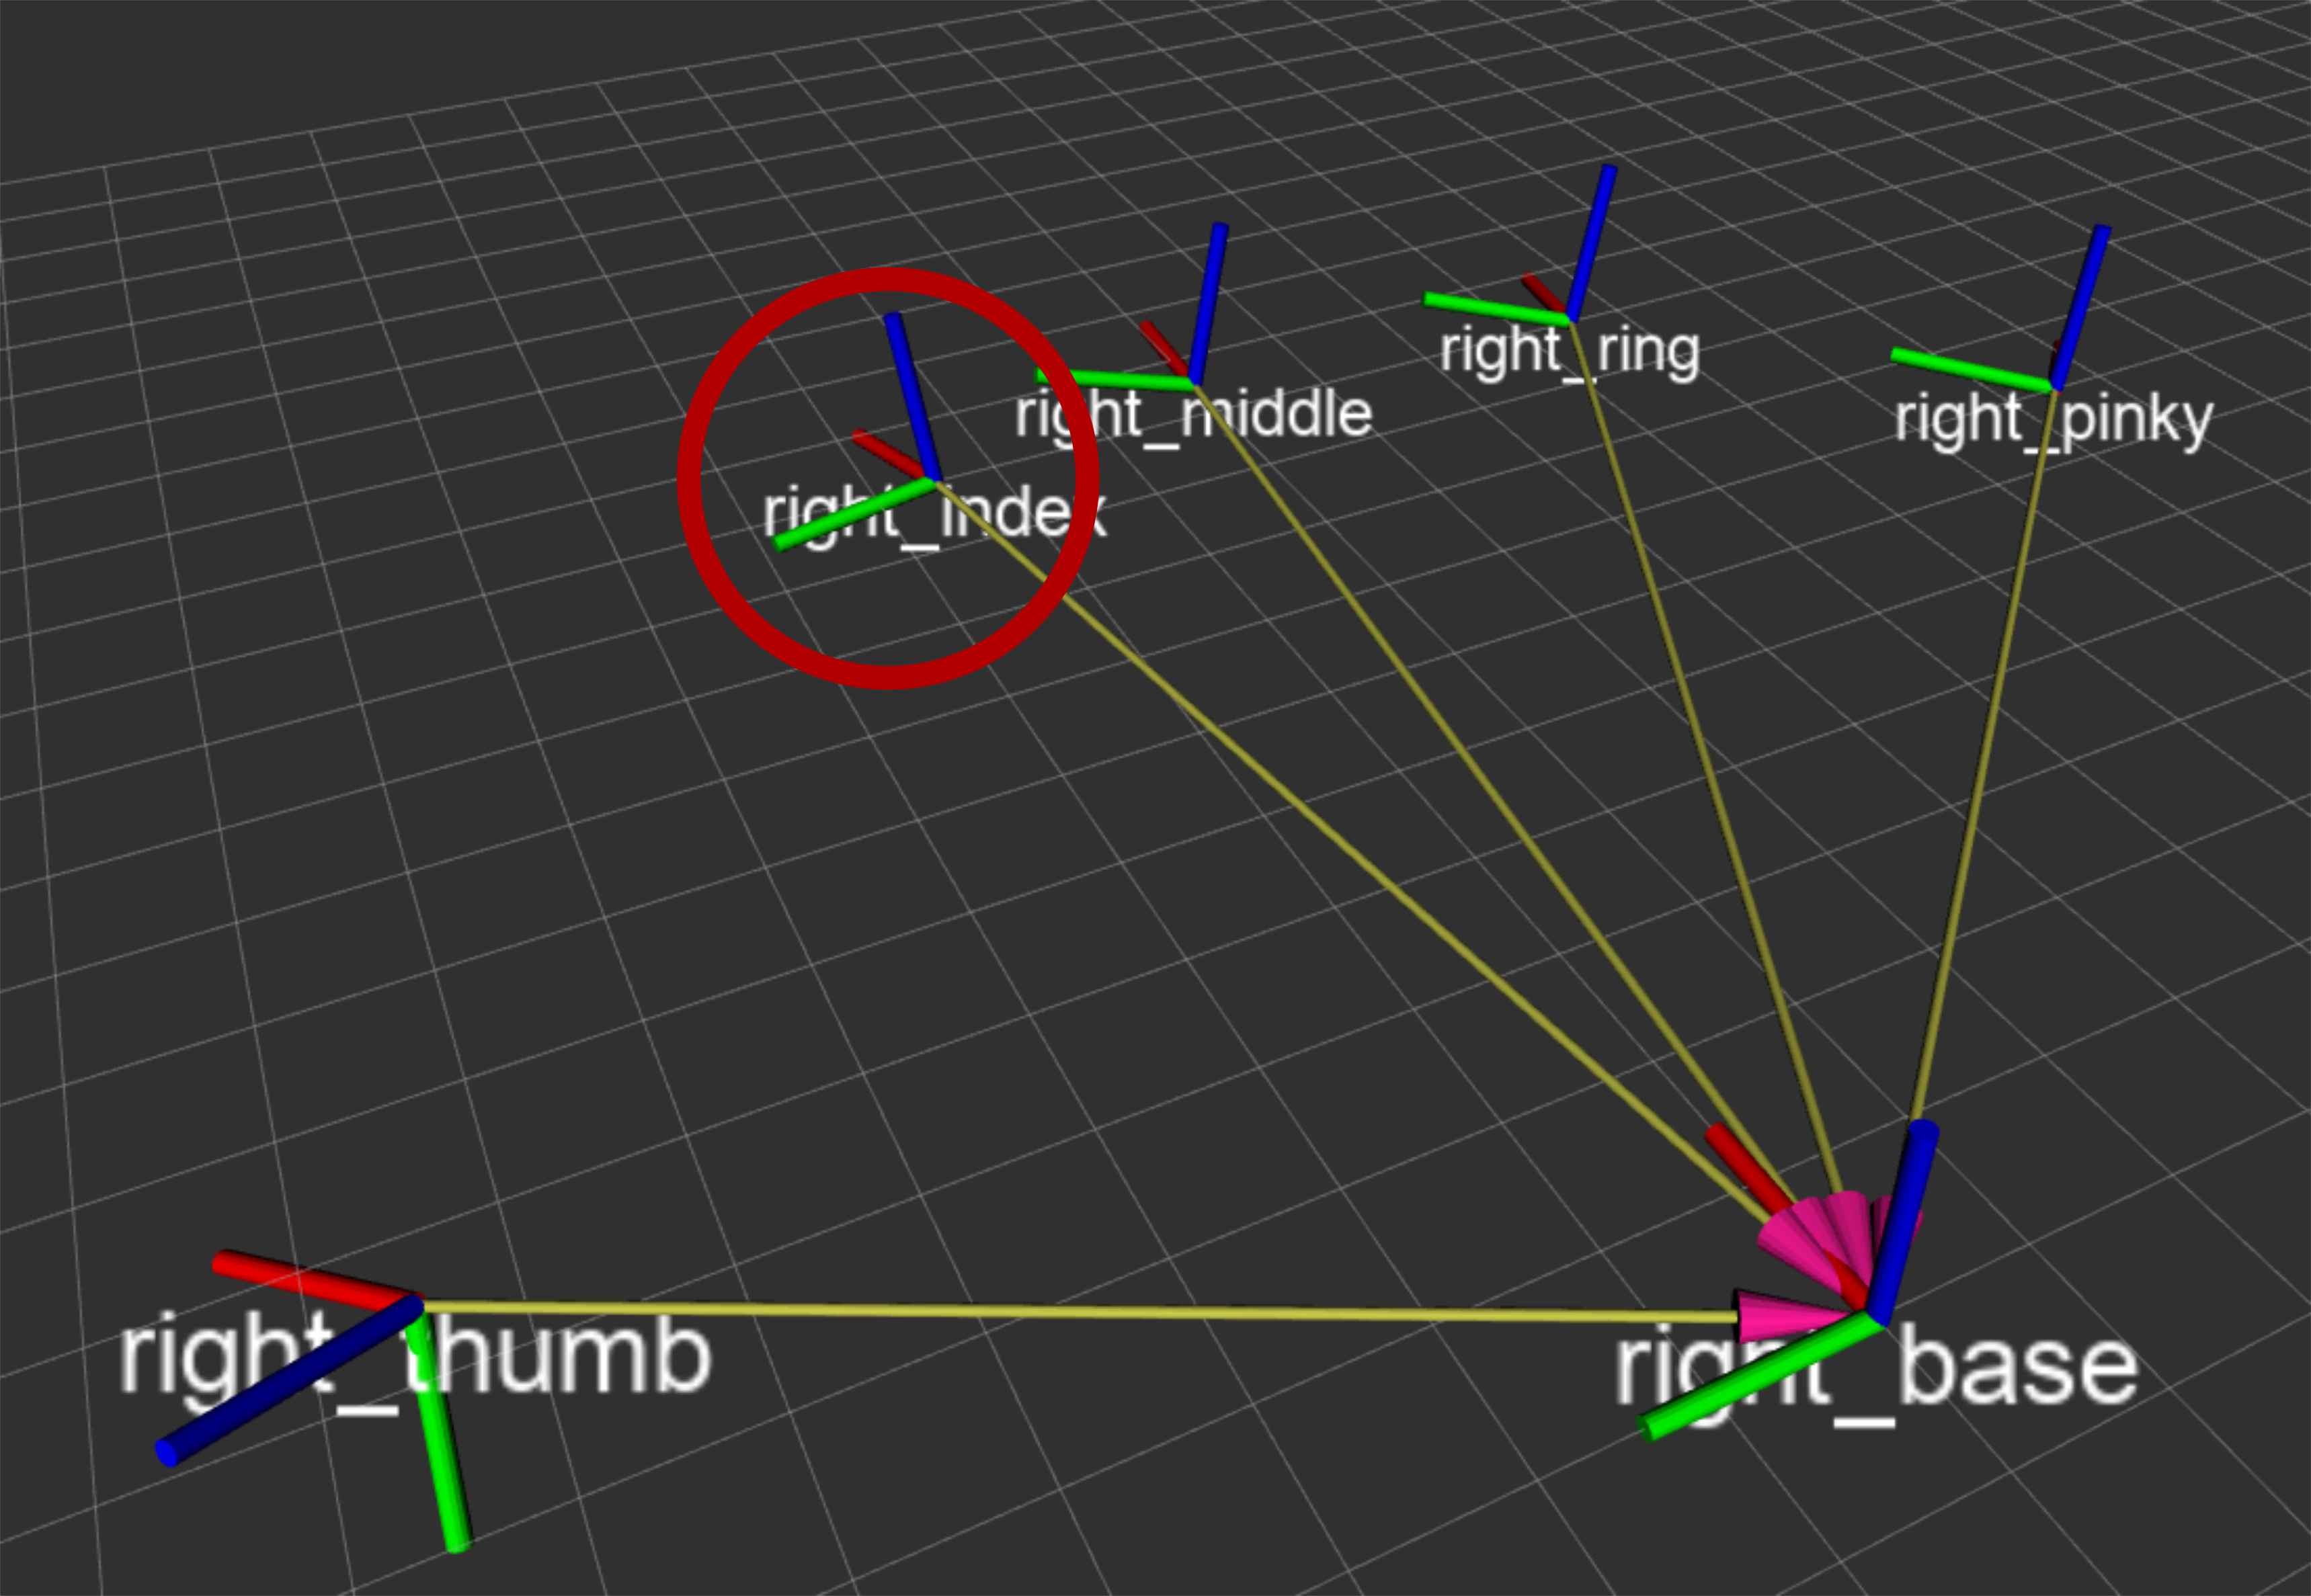
\includegraphics[width=\textwidth]{../common/images/rviz-idle-pose}
        \caption{Alle Finger sind gerade gestreckt.}
        \figlabel{rviz:idle}
    \end{subfigure}
    \hfill
    \begin{subfigure}[t]{0.49\textwidth}
        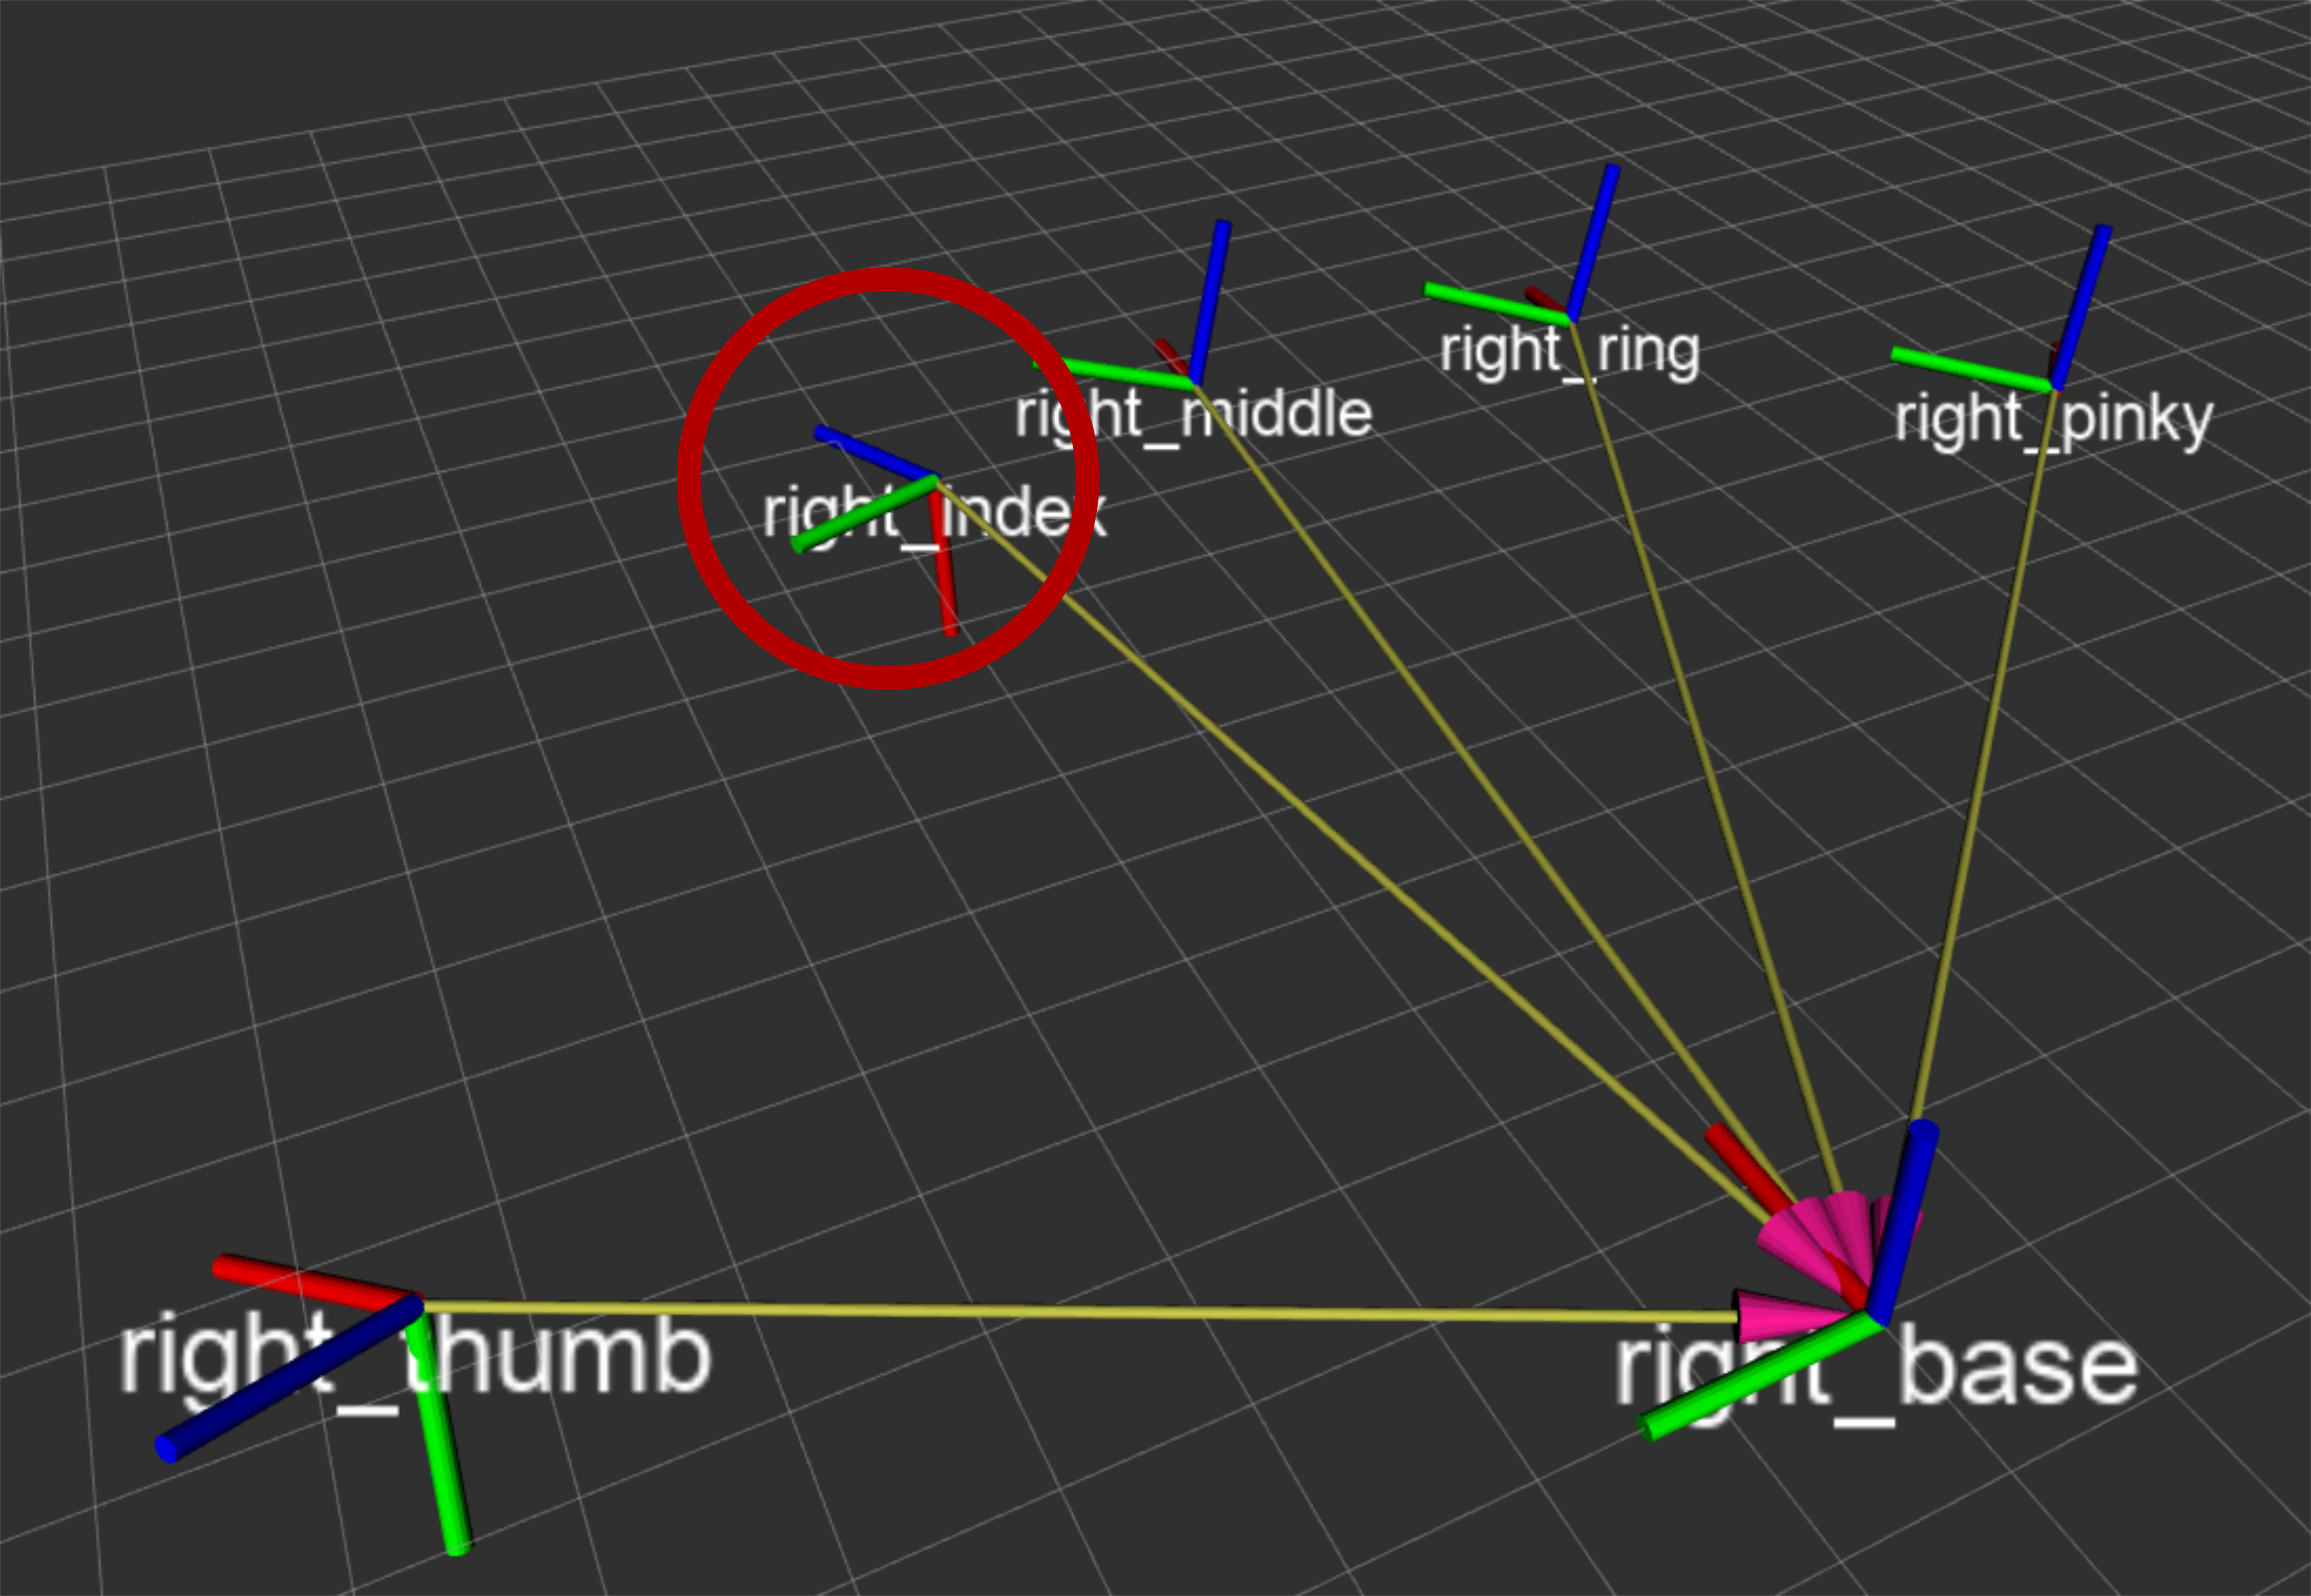
\includegraphics[width=\textwidth]{../common/images/rviz-index-finger-bent}
        \caption{Der Zeigefinger wird gebeugt, die restlichen Finger bleiben gestreckt.}
        \figlabel{rviz:bent}
    \end{subfigure}
    \caption[Darstellung der Hand- und Fingerorientierung]{Darstellung der Hand- und Fingerorientierungen mithilfe des ROS-Visualisierungs-Werkzeugs ,,RViz''. Für die Darstellung wurden vordefinierte Sensorpositionen verwendet, welche jedoch nicht für den Lernvorgang benutzt werden.}
    \figlabel{rviz}
\end{figure}

Um Rückschlüsse auf die Fingerbewegungen machen zu können, berechnen wir die Quaternionen der Finger relativ zu der Quaternion der Hand-IMU. Relative Quaternionen erhält man durch die Multiplikation mit der Inversen der Bezugsorientierung:

$$Q_{\text{rel}}^{\text{finger}} =  Q_{\text{abs}}^{\text{finger}} \cdot inverse(Q_{\text{abs}}^{\text{basis}})$$

\figref{rviz} zeigt einen Screenshot von dem ROS-Visualisierungs-Werkzeug RViz, bei dem der Zeigefinger bewegt wird.
In \figref{rviz:idle} sind sowohl der Zeigefinger als auch die anderen Finger gestreckt.
Beim Abknicken des Zeigefingers ist in \figref{rviz:bent} der relative Winkel der IMU des Zeigefingers zur IMU auf dem Handrücken zu erkennen.

Die Hand-IMU wird relativ zu ihrem gleitenden Mittelwert errechnet. Der gleitende Mittelwert wird verwendet, um einen lokalen Durchschnittswert zu ermitteln. Die zuletzt erfassten Werte werden darin am stärksten gewichtet. Änderungen des Mittelwertes über einen größeren Zeitraum werden also vom gleitenden Mittelwert erfasst, schnelle Änderungen jedoch nicht.

Der gleitende Mittelwert wird wie folgt berechnet:

$$X_{avg}^i = lerp\left(X_{avg}^{i-1}, X^t, \left(t^{i} - t^{i-1}\right) \cdot r\right)$$

$X^i$ ist der Wert und $X_{avg}^i$ der gleitende Mittelwert im
Zeitschritt $i$, $t^i$ ist die tatsächliche Zeit während des  Zeitschrittes $i$, die Anpassungsrate wird als $r$ bezeichnet. Die Funktion $lerp(a, b, f)$ beschreibt die lineare
Interpolation zwischen den Werten $a$ und $b$ im Verhältnis $f$:

$$lerp(a, b, f) := a + (b - a) \cdot f$$

Für Quaternionen verwenden wir statt $lerp$ die sphärische lineare Interpolation $slerp$. Diese berücksichtigt die Interpretation der Quaternion als Angabe für eine Rotation im Raum und interpoliert entsprechend der kürzesten Strecke zwischen zwei Punkten auf der Oberfläche einer Kugel. Das Ergebnis ist wieder eine Einheitsquaternion, die die Teilrotation angibt \citep{spherical_interpolation}.

Das Berechnen der relativen Quaternionen hat mehrere Vorteile:
\begin{enumerate}
    \item Da das Magnometer das Erdmagnetfeld misst, liefert jede IMU absolut ausgerichtete Werte. Die zur Basis-IMU relativen Quaternionen der Finger-IMUs sind hingegen unabhängig davon, in welche Richtung die Hand zeigt.
    \item Die Quaternionen stehen nicht mehr für jeden Finger einzeln, sondern sind in einen Zusammenhang gebracht. Die Fingerbewegung ist unabhängig von der Handbewegung erkennbar. Wird nur die komplette Hand bewegt, aber nicht die einzelnen Finger, ist keine Veränderung an den Daten der Finger erkennbar.
    \item Um auch die Basis-IMU von der absoluten Orientierung unabhängig zu erhalten, haben wir den gleitenden Mittelwert als Bezug gewählt. Dieser passt sich langsam der durchschnittlichen Orientierung der Hand an. Dadurch ist es möglich, zwischen Handbewegungen zu unterscheiden, welche für das Drücken entfernter Tasten nötig sind und solchen, die einer Positionsveränderung beim Schreiben dienen.
    % \item Die Ausrichtungssensibilität der Finger-Quaternionen wird dadurch entschärft. Es ist dadurch nicht lernrelevant, mit welcher Ausrichtung die Daten aufgezeichnet wurden.
    % \item
\end{enumerate}


\subsection{Fester Zeitschritt und Interpolation}

\begin{figure}
    \centering
    \begin{tikzpicture}[
    curve/.style={
        mark=x,
        mark options={thick},
        mark size=3pt,
        thick,
    },
    dot/.style={
        minimum width=4pt,
        minimum height=4pt,
        inner sep=0pt,
        circle,
        draw=secondary,
        thick,
    },
]
    \begin{axis}[
        width=12cm,
        height=6cm,
        axis x line=center,
        axis y line=center,
        xmin=2, xmax=7,
        ymin=2, ymax=5,
        xlabel=Zeit, xtick style={draw=none}, xtick=\empty,
        ylabel=Wert, ytick style={draw=none}, ytick=\empty,
        xlabel near ticks,
        ylabel near ticks,
        legend columns=-1,
        legend style={
            at={(0.5,1.1)},
            anchor=south,
            draw=none,
            font=\scriptsize\bfseries,
            text width=3em,
            text height=1.5ex,
            text depth=.5ex,
        },
    ]
        \addplot[curve,name path=imu-1,color=plot0] plot coordinates {
(-1.90, 1.78) (-1.40, 2.09) (-0.90, 2.32) (-0.40, 2.45) (0.10, 2.58) (0.60, 2.87) (1.10, 3.01) (1.60, 3.01) (2.10, 2.89) (2.60, 2.96) (3.10, 3.05) (3.60, 2.97) (4.10, 2.81) (4.60, 2.77) (5.10, 2.72) (5.60, 2.64) (6.10, 2.49) (6.60, 2.48) (7.10, 2.67) (7.60, 2.81) (8.10, 3.10) (8.60, 3.31) (9.10, 3.48) (9.60, 3.70) (10.10, 3.88) (10.60, 4.05) (11.10, 4.35) (11.60, 4.50)
        };
        \addlegendentry{IMU~1}

        \addplot[curve,name path=imu-2,primary,color=plot1] plot coordinates {
(-1.68, 4.84) (-1.18, 4.89) (-0.68, 4.82) (-0.18, 4.62) (0.32, 4.46) (0.82, 4.13) (1.32, 3.88) (1.82, 3.81) (2.32, 3.71) (2.82, 3.49) (3.32, 3.45) (3.82, 3.24) (4.32, 3.19) (4.82, 3.20) (5.32, 3.24) (5.82, 3.09) (6.32, 2.77) (6.82, 2.62) (7.32, 2.39) (7.82, 2.26) (8.32, 2.32) (8.82, 2.32) (9.32, 2.47) (9.82, 2.55) (10.32, 2.47) (10.82, 2.23) (11.32, 1.92) (11.82, 1.46)
        };
        \addlegendentry{IMU~2}


        \foreach \x/\s [count=\i] in {3.5/2-, 1.5/3-, 5.5/3-, 7.5/3-} {
            \addplot [secondary, name path=line-\i] coordinates{(\x, -0.5) (\x, 5)};

            \path[name intersections={of=imu-1 and line-\i,by=I-\i}];
            \node[dot] at (I-\i) {};

            \path[name intersections={of=imu-2 and line-\i,by=J-\i}];
            \node[dot] at (J-\i) {};
        }

        \draw[secondary,thick,<->]
            (axis cs:3.5,4.6)
                -- node[above] {\tiny{}fester Zeitschritt}
                node[below] {\tiny{}($25$ Hz)}
                (axis cs:5.5,4.6);
    \end{axis}
\end{tikzpicture}

    \caption[Interpolation der IMU-Daten]{Interpolation der IMU-Daten. Die IMUs senden mit \SI{100}{\hertz}, die festen Zeitschritte zu denen neue Daten benötigt werden haben jedoch eine Frequenz von \SI{25}{\hertz}. Durch Interpolation werden die benötigten Daten ermittelt. Dies erfordert das Abwarten der nachfolgenden Datenpunkte.}
    \figlabel{interpolation}
\end{figure}

% \todo wir brauchen Zeitdiskrete daten für das NN. Darum machen wir Zeitschritte in feste Intervallen, und ermitteln die Werte aller Sensoren zu diesem Zeitpunkt. Allerdings senden die IMUs nicht gleichzeitig ihre Werte. Darum verwenden wir Interpolation, um die Zustände zwischen den Sendezeitpunkten zu ermitteln.

Wir haben uns bei der Datenerhebung für die einfache Variante eines festen Zeitschrittes entschieden. Zeitschritte, welche je nach Datenaufkommen kürzer oder länger (also dynamisch) sind, können zwar besser mit bewegungsintensiven beziehungsweise ruhigen Phasen umgehen, benötigen jedoch eine aufwändigere Implementation.

Da die Datenübertragung aller IMUs nicht synchron stattfindet, kommt es vor, dass zu einem festen Zeitschritt die aktuellen Daten der IMUs fehlen. Um trotzdem eine präzise Berechnung zu ermöglichen, versuchen wir die Daten der IMUs möglichst genau anzunähern. Das Vorgehen, welches wir hierfür benutzen, nennt sich Interpolation.

In \figref{interpolation} sind beispielhaft zwei Zeitschritte sowie zwei Wertekurven zu sehen. Um zum Zeitpunkt des Zeitschrittes die aktuellen Werte zu bekommen nutzen wir lineare Interpolation zwischen dem vorherigen und dem nachfolgenden Wert. Für Quaternionen verwenden wir erneut die sphärische lineare Interpolation.

Um den auf den Zeitschritt folgenden Wert für jede IMU zu erhalten und korrekt interpolieren zu können, müssen wir zunächst darauf warten, dass alle IMUs neue Werte gesendet haben. Da die Zeitschritte mit einer Frequenz von 25 Hz stattfinden, die IMUs jedoch mit einer Rate von knapp 100Hz senden, ist diese Wartezeit relativ gering, sie beträgt höchstens \SI{10}{ms}.


\subsection{Sampling (CNN)}

Für den Ansatz mit dem CNN teilen wir die Datenströme in Samples auf. Jedes Sample enthält eine feste Anzahl an Zeitschritten vor und nach einem Tastendruck. Für die Samples der Klasse $\emptyset$ werden die selbe Anzahl aufeinanderfolgender Zeitschritte verwendet, jedoch aus einem Zeitabschnitt, in dem kein Tastendruck vorhanden ist.

Bisher befanden sich die Tastendrücke in der Mitte der Samples, es ist jedoch denkbar, die Anzahl der Zeitschritte nach dem Tastendruck zu reduzieren. Dadurch würde die Verzögerung veringert, die bei der Anwendung des gelernten Netzes durch das Warten auf die restlichen Zeitschritte entsteht.

\section{Visualisierung der Daten}

Um genau zu sehen, mit welchen Daten wir es zu tun haben, beziehungsweise auf welchen Daten das CNN lernen soll, haben wir die Winkel \fremdwort{Yaw} und \fremdwort{Pitch} aus den Quaternionen extrahiert.
% Yaw bezeichnet die Rotation um die vertikale Achse, Pitch die um die \todo
\fremdwort{Roll} ist in unserem Fall ausschließlich für die Hand-IMU, nicht aber für die Finger-IMUs von Interesse, da die Handkinematik ein Rollen der Finger relativ zur Hand nicht ermöglicht.


Zum Visualisieren haben wir die Daten genau wie für das Lernen in Samples geteilt und diese mithilfe der Bibliothek Matplotlib \citep{matplotlib} übereinander gezeichnet, sodass jeweils ein Tastenanschlag am Zeitpunkt 0 angeordnet war. Das Ergebnis ist in \figref{plot-samples} zu sehen.

Wir haben diese Graphen für verschiedene Finger- und Tastenkombinationen erstellt. Die entstehenden Muster sind für die verschiedenen Tasten gut unterscheidbar, daher konnten wir davon ausgehen, dass auch ein ML-Algorithmus dazu in der Lage sein würde, sie zu unterscheiden.

\begin{figure}
    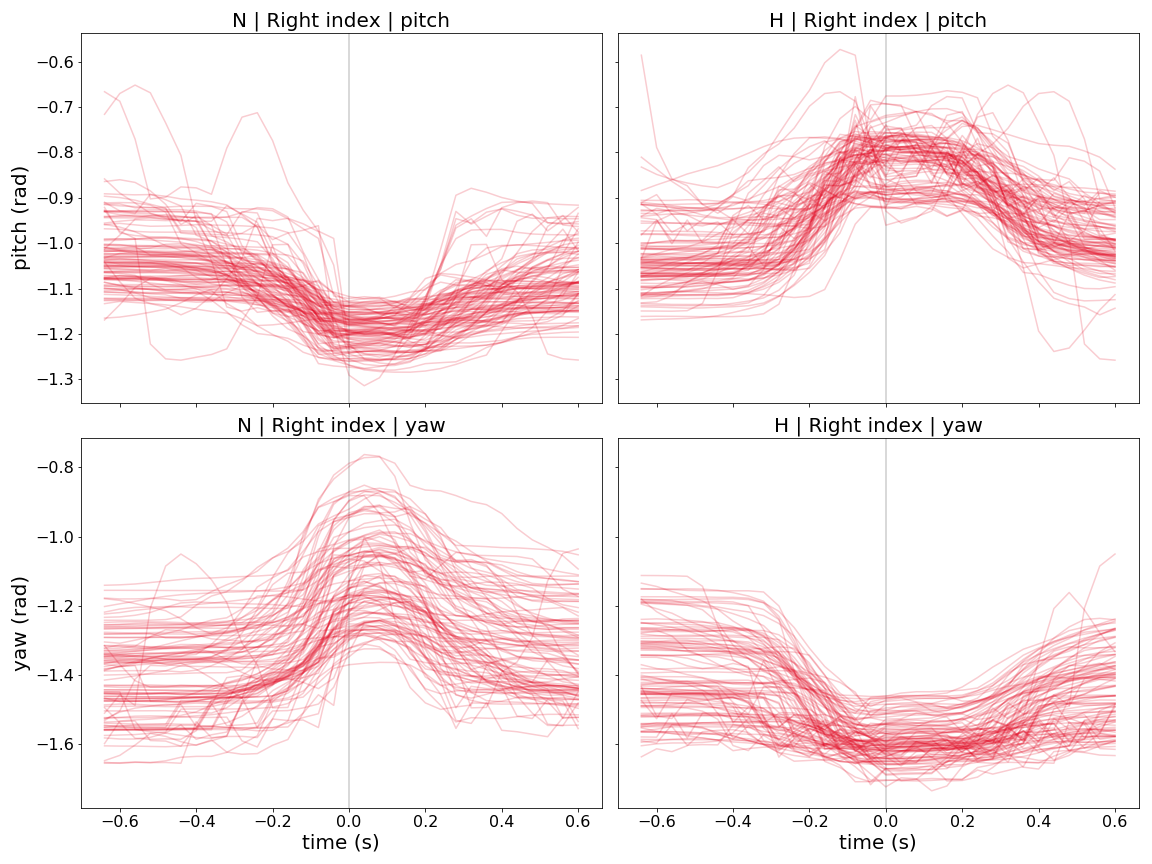
\includegraphics[width=\textwidth]{../common/images/plot-samples-2x2.png}
    \caption[Mehrfache Wiederholungen eines Tastendrucks]{Mehrfache Wiederholungen des Drückens der Taste \keyboard{N} (links) und \keyboard{H} (rechts), im Moment des Tastendrucks übereinander gelegt. Zu sehen sind jeweils der extrahierte Pitch- (oben) und Yaw-Winkel (unten) des rechten Zeigefingers.}
    \figlabel{plot-samples}
\end{figure}

\section{Netzarchitektur}

Dieser Abschnitt behandelt die Konfiguration der verwendeten neuronalen Netze. Es wird zunächst die Konfiguration des RNN beschrieben, anschließend wird auf die Konfiguration des CNN eingegangen.

\subsection{Recurrent Neural Network}

Unser erster Ansatz für eine Netzarchitektur basierte auf einem RNN. Hiermit versprachen wir uns, die Bewegungsabläufe effizient lernen zu können, da RNNs für sequezielle Daten geeignet sind. Wir stießen recht schnell auf diverse Probleme.
%Ein Problem war, eine geeignete Methode zu finden, mit den vom Handschuh erhaltenen Daten, welche wir vom Datenhanschuh erhalten, sinnvoll lernen zu können.
Ein Problem, welches man oft bei der Nutzung eines RNN lösen muss, ist das \fremdwort{vanishing gradient problem} \citep{hochreiter-vanishing-gradient}. Es bezeichnet das Phänomen, dass die vorderen Kanten eines Netzes kaum angepasst werden, da der ermittelte Anteil am gemachten Fehler vor allem auf die der Ausgabeschicht nahen Kanten verteilt werden. Da ein RNN meist ein sehr tiefes Netz ist, verschwindet der Anteil immer weiter, die ersten Kanten akkurat zu trainieren dauert dementsprechend lange.

Ein weiteres Problem entsteht durch die Struktur der Daten, mit welchen wir das Netz trainieren.
Unsere Aufgabenstellung ist ein Klassifikationsproblem mit mehreren Klassen. Die positiven Klassen beinhalten ausschließlich die Zeitpunkte, zu denen gerade eine Taste hiuntergedrückt wird. Die große, negative Klasse beinhaltet alle Zeitpunkte, in denen eine gedrückte Taste im Vorfeld bereits gedrückt war, oder aber in denen gar keine Taste gedrückt ist. Es handelt sich um stark unbalancierte Daten, wie sie in \chapref{grundlagen} bereits beschrieben werden.

Dort wurden auch verschiedene Methoden vorgestellt, um mit unbalancierten Daten umzugehen.

Leider erwiesen sich diese als nur bedingt geeignet für unseren Anwendungsfall.
Unsere Daten stellen Bewegungsabläufe dar, welche von dem RNN auch als solche gelernt werden sollen. Es ist nicht möglich, die Daten in einzelne Sequenzen zu teilen, ohne genau zu wissen, an welcher Stelle man die Daten teilen kann, ohne einen zusammengehörenden Bewegungsablauf zu durchtrennen. Resampling war demnach nicht möglich.

Auch bei der Verwendung diverser bestrafender Kostenfunktionen erzielten wir kein gutes Ergebnis. Lasagne bietet einige bereits implementierte Kostenfunktionen, welche falsches Klassifizieren unterschiedlich stark gewichten. Leider konnten wir jedoch keine Kostenfunktion finden, welche eine signifikante Verbesserung des Lernens erbrachte.

Nach der ersten Versuchs-Phase (\secref{phase1}) entschieden wir uns dazu, ein anderes neuronales Netz zu verwenden und zusätzlich die Vorverarbeitung der Daten zu verbessern.

\subsection{Convolutional Neural Network}
\subseclabel{cnn}

\begin{figure}
    \centering
    \begin{tikzpicture}[
    node distance=5mm,
    node/.style={
        flowchart node,
        minimum width=3em,
        text width=3em,
    },
    steplabel/.style={
        font=\scriptsize,
        below,
        anchor=north,
    },
    arrow/.style={
        out=-30,
        in=210,
    },
]
    \node[node] (data) {1 @\\16 x 24};
    \node[node, right=of data] (conv1)  {50@\\$16\times24$};
    \node[node, right=of conv1] (pool1) {50@\\$8\times12$};
    \node[node, right=of pool1] (conv2) {50@\\$8\times12$};
    \node[node, right=of conv2] (pool2) {50@\\$4\times6$};
    \node[node, right=of pool2] (hidden) {Hidden\\Layer};
    \node[node, right=of hidden] (out) {Output\\Layer};

    \draw[flowchart arrow,shorten >=2pt] (data.south)   to[arrow] node[steplabel] {Convolution 1} (conv1.south);
    \draw[flowchart arrow,shorten >=2pt] (conv1.south)  to[arrow] node[steplabel] {Pooling 1} (pool1.south);
    \draw[flowchart arrow,shorten >=2pt] (pool1.south)  to[arrow] node[steplabel] {Convolution 2} (conv2.south);
    \draw[flowchart arrow,shorten >=2pt] (conv2.south)  to[arrow] node[steplabel] {Pooling 2} (pool2.south);
    \draw[flowchart arrow,shorten >=2pt] (pool2.south)  to[arrow] node[steplabel] {Dense 1} (hidden.south);
    \draw[flowchart arrow,shorten >=2pt] (hidden.south) to[arrow] node[steplabel] {Dense 2} (out.south);
\end{tikzpicture}

    \caption[Architektur des verwendeten CNN]{Die Architektur des verwendeten CNN. Es ist die Veränderung in der Anzahl und der Größe der Feature Maps zu sehen, welche durch die abwechselnden Convolution- und Poolingschritten entstehen.}
    \figlabel{cnn-flowchart}
\end{figure}

Wir änderten die Netzwerkarchitektur und verwendeten nun ein CNN. Ein großer Vorteil ist hierbei, dass die Erkennung der Muster auf festen Zeitabschnitten möglich ist, es ist also nicht mehr nötig, zusammenhängende Sequenzen zu lernen. Somit konnten wir die Daten recht leicht in die verschiedenen Samples teilen, wodurch auch das Resampling erleichtert wurde. Für jede zu lernende Taste wurden ähnlich viele Tastendrücke aufgezeichnet. Dadurch waren die Klassen der Tastendrücke gleichmäßig verteilt. Um auch die Klasse $\emptyset$ lernen zu können, fügten wir zu den Tasten-Samples entsprechend viele weitere Samples hinzu, in denen kein Tastendruck enthalten war. Hierbei achteten wir darauf, einen Minimalabstand zu den Tastendrücken einzuhalten, damit die Klasse $\emptyset$ auch keine Tastendrücke am Rand der Samples enthält.

Wir arbeiten mit der in \figref{cnn-flowchart} gezeigten Netzstruktur.
Die Eingabedaten sind die Quaternionen aller 6 IMUs zu den festen Zeitschritten. Diese ergeben eine \num{16 x 24} große Eingabematrix, bei einer Samplegröße von 16 Zeitschritten. Der Tastendruck befindet sich in der Mitte der Zeitschritte.

Mithilfe der 50 Filter werden 50 Feature Maps der gleichen Dimension erzeugt. Beim Pooling werden diese Feature Maps dann auf die Größe \num{8x12} reduziert. Der nächste Convolution-Schritt führt wiederum zu 50 Feature Maps. Dass sich die Anzahl der Feature Maps nicht erhöht, liegt daran, dass jeder Filter alle vorherigen Feature Maps verwendet. Die Filter haben also die Form \num{3x3x50}.

Nach dem nächsten Pooling-Schritt werden die Feature Maps in die erste versteckte Schicht des einfachen Klassifikators gereicht und von dort aus wird in der Ausgabeschicht die Klasse ermittelt.

\begin{figure}
    \centering
    \begin{subfigure}[t]{0.49\textwidth}
        \centering
        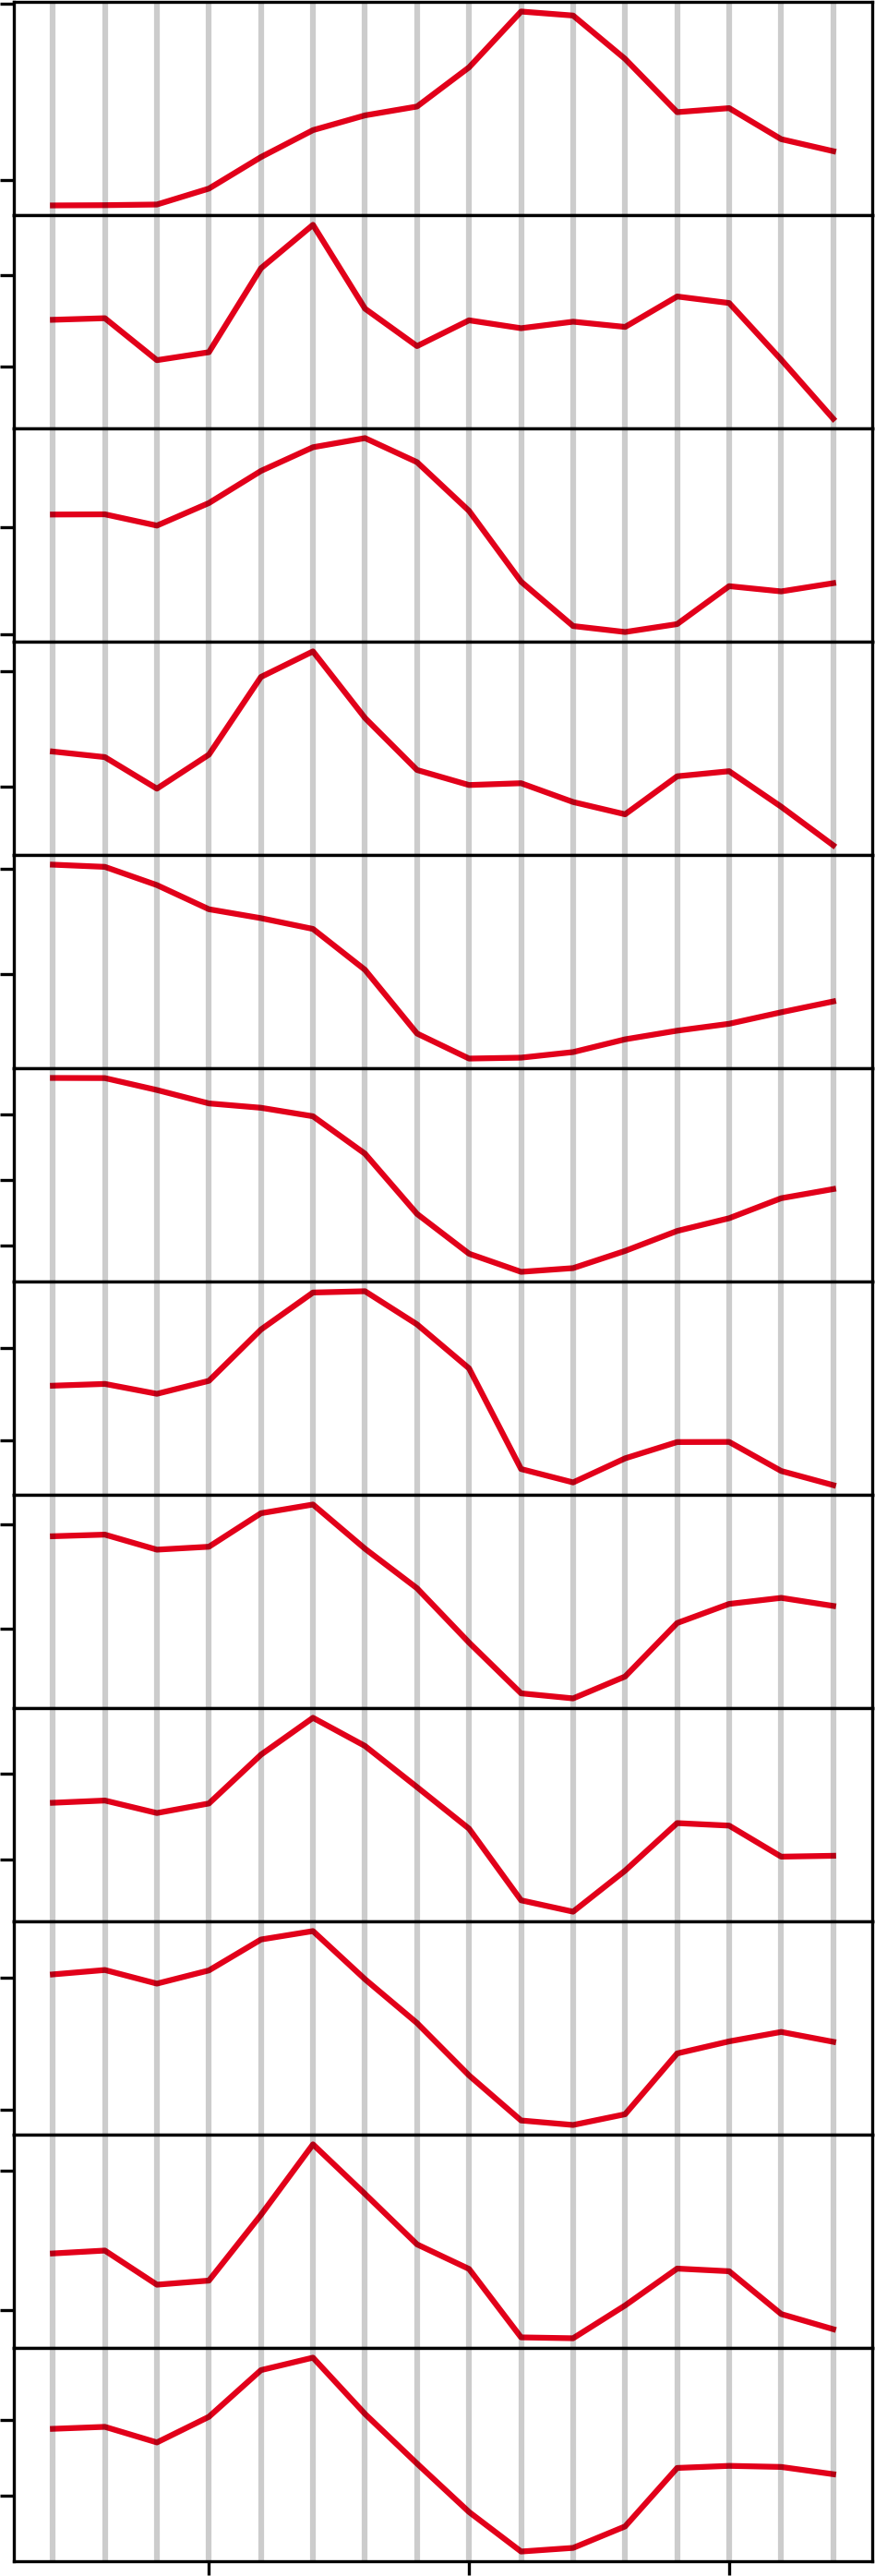
\includegraphics[width=4cm,height=6cm]{../common/images/input-plot}
        \caption{Einzelwerte, hier Pitch- und Yaw-Winkel, aller IMUs (vertikal) über die 16 Zeitschritte des Samples (horizontal)}
        \figlabel{cnn-input:graphs}
    \end{subfigure}
    \hfill
    \begin{subfigure}[t]{0.49\textwidth}
        \centering
        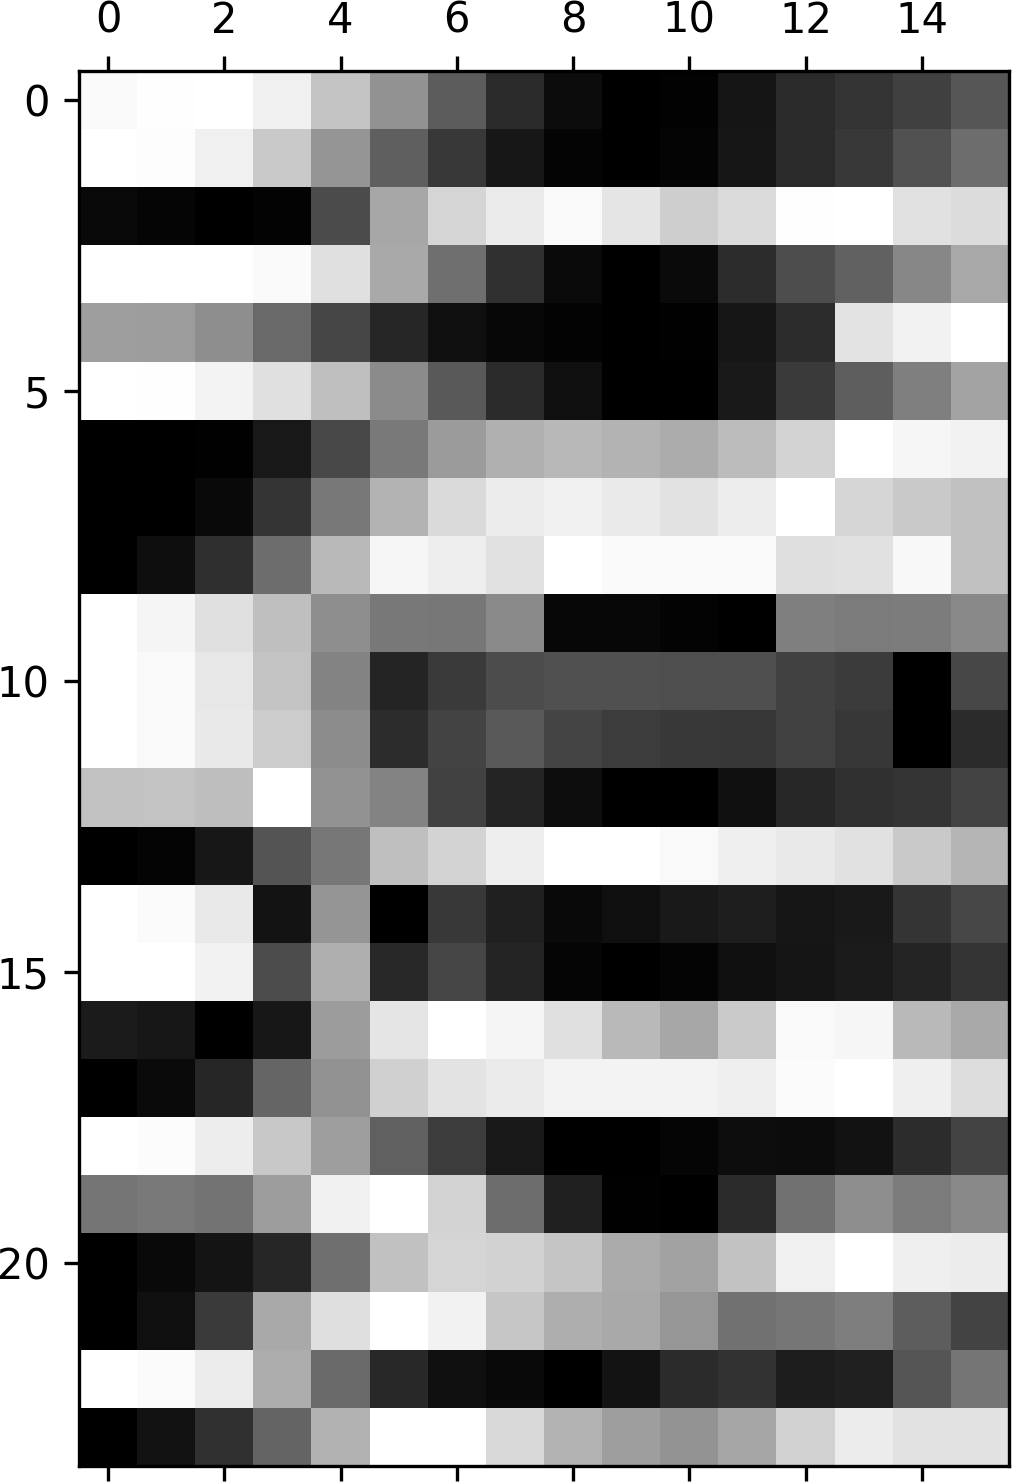
\includegraphics[width=4cm,height=6cm]{../common/images/input-matrix}
        \caption{Alternative Darstellung der Eingabewerte, hier die kompletten Quaternionen als Datenmatrix (zeilenweise normalisiert). Jede Zeile in der Matrix entspricht einem Einzelwert, jede Spalte einem der 16 Zeitschritte.}
        \figlabel{cnn-input:matrix}
    \end{subfigure}

    \caption{Eingabedaten für das CNN auf verschiedene Arten visualisiert.}
    \figlabel{cnn-input}
\end{figure}

In \figref{cnn-input} sind die Eingabedaten des CNN zu sehen. In \figref{cnn-input:graphs} wurden aus den Quaternionen die Yaw- und Pitch-Winkel extrahiert, da diese visuell leichter zu deuten sind als ganze Quaternionen, welche eigentlich für das Lernen genutzt werden. Ein Sample besteht aus 16 Zeitschritten und beinhaltet die kompletten Quaternionen, also pro IMU 4 Werte.
In \figlabel{cnn-input:matrix} sind die Eingabedaten, in diesem Fall tatsächliche Quaternionen, als Graustufenmatrix gezeigt. Jedes Sample ist eine solche Matrix, die Eingabeschicht des CNN hat eine entsprechende Form.

% Hier Grafik mit dem Layer-Größen rein.


\section{Konfiguration}
\seclabel{konfig}

Der Aufbau des neuronalen Netzes bietet viele Variablen, die sein Verhalten beeinflussen. Diese Variablen müssen angepasst werden, um für den Anwendungsfall optimale Eigenschaften zu erhalten.

Um Experimente nachvollziehbar und wiederholbar und die verschiedenen Konfigurationen leicht veränderbar zu gestalten, wurde eine Konfigurationsdatei angelegt (siehe \lstref{config}), deren Variablen hier vorgestellt werden.

\begin{listing}[h]
    \inputminted{yaml}{../common/code/config.yaml}
    \caption[Konfigurationsdatei]{Konfigurationsdatei für den Lernprozess. Die Konfigurationsdatei wird geladen und anhand ihrer Einstellungen wird das Verhalten der Software angepasst. Unter anderem können das Lernverhalten, die Netzwerkarchitektur sowie die verwendeten Daten und deren Zerlegung in Samples eingestellt werden.}
    \lstlabel{config}
\end{listing}

\begin{description}[font=\texttt]
    \item[imu\_ids]
        Hier wird definiert, welche IMUs des Handschuhs verwendet werden sollen. Zu Beginn des Projektes wurden oft nur eine oder zwei IMUs benötigt, um die Daten, welche die IMUs liefern zu analysieren.

    \item[key\_codes]
        Die Key Codes der zu lernenden Tasten stammen vom  Linux Input Event System\footnote{in einem Linux Betriebsystem unter \texttt{/usr/include/linux/input-event-codes.h} einzusehen}. Diese Variable beeinflusst, welche Tasten das neuronalen Netz zu erkennen lernt. Anhand ihrer wird die Größe der Ausgabeschicht ermittelt. Sie ist außerdem in der Anwendung des gelernten Modells nötig, um die Ausgaben in Tastendrücke zurück zu übersetzen.

    \item[sequence\_length]
        Mit der Länge der Sequenz wird die Anzahl der verwendeten Zeitschritte pro Sample festgelegt.

    \item[sequence\_ratio]
        Durch diese Variable wird die Verteilung der Zeitschritte vor und nach dem Tastendruck bestimmt. Bisher haben wir eine gleichmäßige Aufteilung gewählt, es ist jedoch denkbar, die Anzahl der Zeitschritte nach einem Tastendruck zu verringern, um entstehende Verzögerungen zu reduzieren.

    \item[sampling\_mode]
        Hier wird festgehalten, welche Daten zum Lernen verwendet werden. Mögliche Ausprägungen sind \texttt{quat}, \texttt{angles} und \texttt{full}. Bisher lernen wir ausschließlich auf den Quaternionen, im weiteren Verlauf könnte es aber sinnvoll sein, die rohen Daten des Accelerometers und des Gyroskops ebenfalls zu verwenden.

    \item[sampling\_rate]
        Die Frequenz der Zeitschritte wird in Hertz angegeben und bestimmt die Abstände der Zeitpunkte, in denen die IMU-Daten gebündelt und aufgezeichnet werden.
        Wenn zu den Quaternionen weitere Werte zum Lernen verwendet werden, kann es sinnvoll sein, eine höhere Frequenz zu verwenden.

    \item[base\_imu\_relative\_average\_rate]
        Dieser Wert bezeichnet die Anpassungsrate des gleitenden Mittelwertes der Hand-IMU. Hierfür haben wir experimentell den Wert $r = 0.2$ als geeignet ermittelt.

    \item[epochs]
        Mit dieser Einstellung lässt sich bestimmen, wie viele Epochen ein Netz lernen soll. Der Wert 0 besagt hier, dass solange immer weitere Epochen gelernt werden sollen, bis der Vorgang abgebrochen wird.

    \item[batch\_size]
        Die Stapelgröße, mit der gelernt wird, ist über diese Variable anpassbar. Ein Stapel ist ein Zusammenschluss von in unserem Fall 100 Samples, jede Epoche trainiert mit einem Stapel dieser Größe.

    \item[training\_ratio]
        Das Lernen eines neuronalen Netzes findet mit zwei disjunkten Teilen eines Datensatzes statt. Der größere Teil ist der Trainingsdatensatz. Dieser wird benutzt, um das Netz zu trainieren. Der andere Teil des Datensatzes ist für die Evaluation vorgesehen. Hierbei wird getestet, ob das Netz das Gelernte auch auf ihm unbekannte Daten anwenden kann, oder ob es die Generalisierungsfähigkeit durch zu starkes Lernen verloren hat. In unserem Fall ist die Aufteilung 0.8, das heißt 80\% der Daten stehen als Trainingsdaten zur Verfügung, der Rest wird zum Testen verwendet.

    \item[cost\_function]
        Die Kostenfunktion errechnet den Fehler der Ausgabe eines neuronalen Netzes. Wir verwenden den \fremdwort{Mean Squared Error} (MSE). Diese einfache Kostenfunktion ist für das CNN  ausreichend, da auf einem balancierten Datensatz gelernt wird. Beim RNN testeten wir viele verschiedene Kostenfunktionen aus, um trotz unbalanciertem Datensatz eine gute Genauigkeit zu erreichen, ohne die unterrepräsentierten Klassen zu übergehen.

    \item[network\_type]
        Hier kann zwischen den zwei verschiedenen Netztypen gewählt werden, einem RNN oder einem CNN.

    \item[learning\_rate]
        Die Lernrate eines neuronalen Netzes bezeichnet den Grad der Anpassung anhand der Fehlerrate.
        Eine zu geringe Lernrate bewirkt, dass das Netz Anpassungen nur sehr langsam vollzieht, das Lernen dauert dementsprechend lange. Ist die Lernrate jedoch zu hoch, kann es passieren, dass nie ein optimal gelerntes Netz erhalten wird, da die Kantengewichtsanpassungen dazu führen, dass über das Ziel hinausgeschossen wird und die Vorhersagen des Netzes zu oszillieren beginnen.
        Wir beginnen mit einer Lernrate von 0.002 und nutzen den AdaGrad-Algorithmus von \citet{adagrad}, um die Lernrate mit vergehender Zeit zu verringern. Dies sorgt dafür, dass spätere Anpassungen nur noch geringe Veränderungen bewirken.

    \item[n\_hidden]
        Bei dieser Variable handelt es sich um die Anzahl der Einheiten innerhalb der versteckten Schicht des RNN.

    \item[convolution\_filter\_count]
        Die Anzahl der Filter pro Convolution-Schritt.

    \item[convolution\_filter\_size]
        Die Filter im CNN haben eine feste Größe. Diese bestimmt den Einfluss der Nachbarschaft auf den vom Filter ermittelten Wert. Wir haben uns für Filter der Größe \num{3 x 3} entschieden.

    \item[convolution\_iterations]
        Ein CNN vollzieht mehrere Iterationen der Convolution- und Poolingschritte. Wir verwendeten 2 Iterationen, ob diese Anzahl genügt, oder ob mehr Iterationen gemacht werden sollten, muss in weiteren Versuchen herausgefunden werden.

    \item[convolution\_dense\_layer\_units]
        Die Anzahl der Einheiten der vollständig verbundenen Schicht zur Klassifizierung am Ende des CNN haben wir zu Beginn auf 10 gesetzt. Da die Ausgabeschicht im weiteren Verlauf der Experimente mehr als 10 Einheiten enthielt, wurde diese Zahl nach oben korrigiert. Diese Variable verwendet eine Liste von Werten, sodass eine beliebige Anzahl vollständig verbundener Schichten unterschiedlicher Größe wählbar ist.

    \item[convolution\_deep\_filters]
        Hier wird ausgewählt, ob tiefe Filters verwendet werden sollen. Tiefe Filter werden auf allen vorherigen Feature Maps angewandt, flache Filter nur auf jeweils einer. Dadurch führen flache Filter zu einer exponentiell wachsenden Anzahl an Feature Maps. Wir verwenden tiefe Filter, im Grunde haben diese ab der zweiten Convolution-Schritt also die Größe \num{3 x 3 x 50}. Dies reduziert die Komplexität des Netzes.
\end{description}


